\documentclass[aspectratio=169]{beamer}
\usepackage[utf8]{inputenc}
\usepackage{amsmath}
%\usepackage[ngerman]{babel}
\usepackage{xcolor}
\usepackage{listings}
%\usepackage[automark]{scrpage2}
\usepackage[]{graphicx, import} 
\usepackage{subfigure}
\usepackage{wrapfig}
\usepackage[scaled]{helvet}
\renewcommand*\familydefault{\sfdefault}
%\usepackage{enumitem}
\usepackage{harvard}
\usepackage{url}
\citationstyle{dcu}
%\setbeamertemplate{footline}[page number]
\usetheme{FHNW}
\usecolortheme{seagull}
\usepackage{multimedia}

\usepackage{hyperref}



\begin{document}
% infos for pdf document settings
\pdfinfo{
/Author (Stefan Blaser, FHNW - IVGI)
/Title (Development of an Acquisition Software 
	for our Image-Based Indoor Mobile Mapping System 
	based on the Robot Operating System (ROS))
/Subject (GeoPython 2017)
/Keywords (ROS, Mobile Mapping, Indoor, Python)}

% infos for title page
\title{\textbf{Development of an Acquisition Software
	for our Image-Based Indoor Mobile Mapping System 
	based on the Robot Operating System (ROS)}}
\subtitle{GeoPython 2017}
\author{Stefan Blaser}
\institute{Institute of Geomatics Engineering}
\date{\today}

% title page
\begin{frame}
 \titlepage
\end{frame}

\section{Introduction}

% Frame 1: Trends in geodata acquisition
  \begin{frame}
   \frametitle{Introduction}
   \begin{columns}[onlytextwidth]
    \begin{column}{0.5\textwidth}
    
    % TODO insert Image (IOT)
    
    \end{column}
    \begin{column}{0.5\textwidth}
    Trends in geodata acquisition:
      \begin{itemize}
       \item outsourcing / crowd-sourcing
       \item IoT
       \item using sophisticated multi-sensor systems
      \end{itemize}
    \end{column}
   \end{columns}
  \end{frame}

% Frame 2: Mobile Mapping
  \begin{frame}
   \frametitle{Introduction}
   \begin{columns}[onlytextwidth]

    \begin{column}{0.5\textwidth}
    Mobile Mapping
      \begin{itemize}
       \item Image-based Mobile Mapping \newline(since 2011 @ FHNW)
       % TODO cite Burkhard et. al (2011)
       \item Spin-off company iNovitas
       \item ``Google Street View''-like service
       \item Measurement functionality
       \item Measurement accuracy:
       \begin{itemize}
        \item relative: ca. $1\, cm$
        \item absolute: ca. $3-5\, cm$ \newline(GNSS accuracy)
       \end{itemize}
      \end{itemize}
    \end{column}
    \begin{column}{0.5\textwidth}
    
     \begin{figure}[h]
       \centering
       \includegraphics[width=5.5cm]{./Abbildungen/mms.png}
       \caption{Mobile Mapping vehicle of FHNW}
       \label{abb:mms}
     \end{figure}
     
    \end{column}
    
   \end{columns}
  \end{frame}

% Frame 3: CTI-Project BIMAGE
  \begin{frame}
   \frametitle{Introduction}
   \begin{columns}[onlytextwidth]

    \begin{column}{0.5\textwidth}
    CTI project ``BIMAGE''
      \begin{itemize}
       \item Main Goal: 
       \begin{itemize}\item Transfer outdoor technology into interior spaces\end{itemize}
       \pause
       \item Deliverables:
       \begin{itemize}
        \item \textbf{Indoor Mobile Mapping System} (IMMS) (absence of GNSS) \pause
        \item Software to follow changes using mobile devices \pause
        \item New navigation concepts for cloud application \pause
        \item Sophisticated photogrammetric image post-processing approaches 
       \end{itemize}
      \end{itemize}
    \end{column}
    \begin{column}{0.5\textwidth}
    \begin{center}
    
\includegraphics[width=0.9\textwidth]{./Abbildungen/FHNW_HABG_10mm.jpg} \\
    % FHNW_HABG_10mm.jpg: 0x0 pixel, 300dpi, 0.00x0.00 cm, bb=
    
\includegraphics[width=0.2\textwidth]{./Abbildungen/iNovitas_Logo.png} \\
    % iNovitas_Logo.png: 0x0 pixel, 300dpi, 0.00x0.00 cm, bb=
    
\includegraphics[width=0.7\textwidth]{./Abbildungen/F&E_Absender_Dritte_Un_D_1200.png}
% F&E_Absender_Dritte_Un_D_1200.png: 0x0 pixel, 300dpi, 0.00x0.00 cm, bb=
    \end{center}
    
    \end{column}
    
   \end{columns}
  \end{frame}


\section{Software Requirements}

  \begin{frame}
   \frametitle{Requirements for the acquisition software}
   \begin{columns}[onlytextwidth]
    \begin{column}{0.5\textwidth}
    
    \begin{figure}[h]
      \centering
      \includegraphics[height=6.05cm]{./Abbildungen/imms.png}
      %\caption{IMMS prototype}
      \label{abb:imms}
    \end{figure}

    \end{column}
    \begin{column}{0.5\textwidth}
      \begin{itemize}
       \item IMMS prototype (see figure)  
       \begin{itemize}
        \item panorama camera
        \item laser scanner
        \item IMU (tactical grade)
        \item GNSS
	\item weight: $30\,kg$ ($66.1\, lbs$)
	\item hardware changes necessary
       \end{itemize}
       \pause
       \item Modular software architecture
       \item Free open source software (FOSS)
       \item Existing modules for hardware support
      \end{itemize}
    \end{column}

   \end{columns}
  \end{frame}

\section{Robot Operating System (ROS)}

  \begin{frame}
   \frametitle{Robot Operating System (ROS)}
   \begin{columns}[onlytextwidth]
    \begin{column}{0.5\textwidth}
    
      \begin{itemize}
       \item Software framework for robots 
       \item Free and Open-Source 
       \item Graph-based communication layer 
       \item Collection of tools and libraries 
       \item Multi-lingual 
       \begin{itemize}
	\item C++
	\item \textbf{Python} 
       \end{itemize}
       \item \url{www.ros.org}
      \end{itemize}
    
    \end{column}
    \begin{column}{0.5\textwidth}

    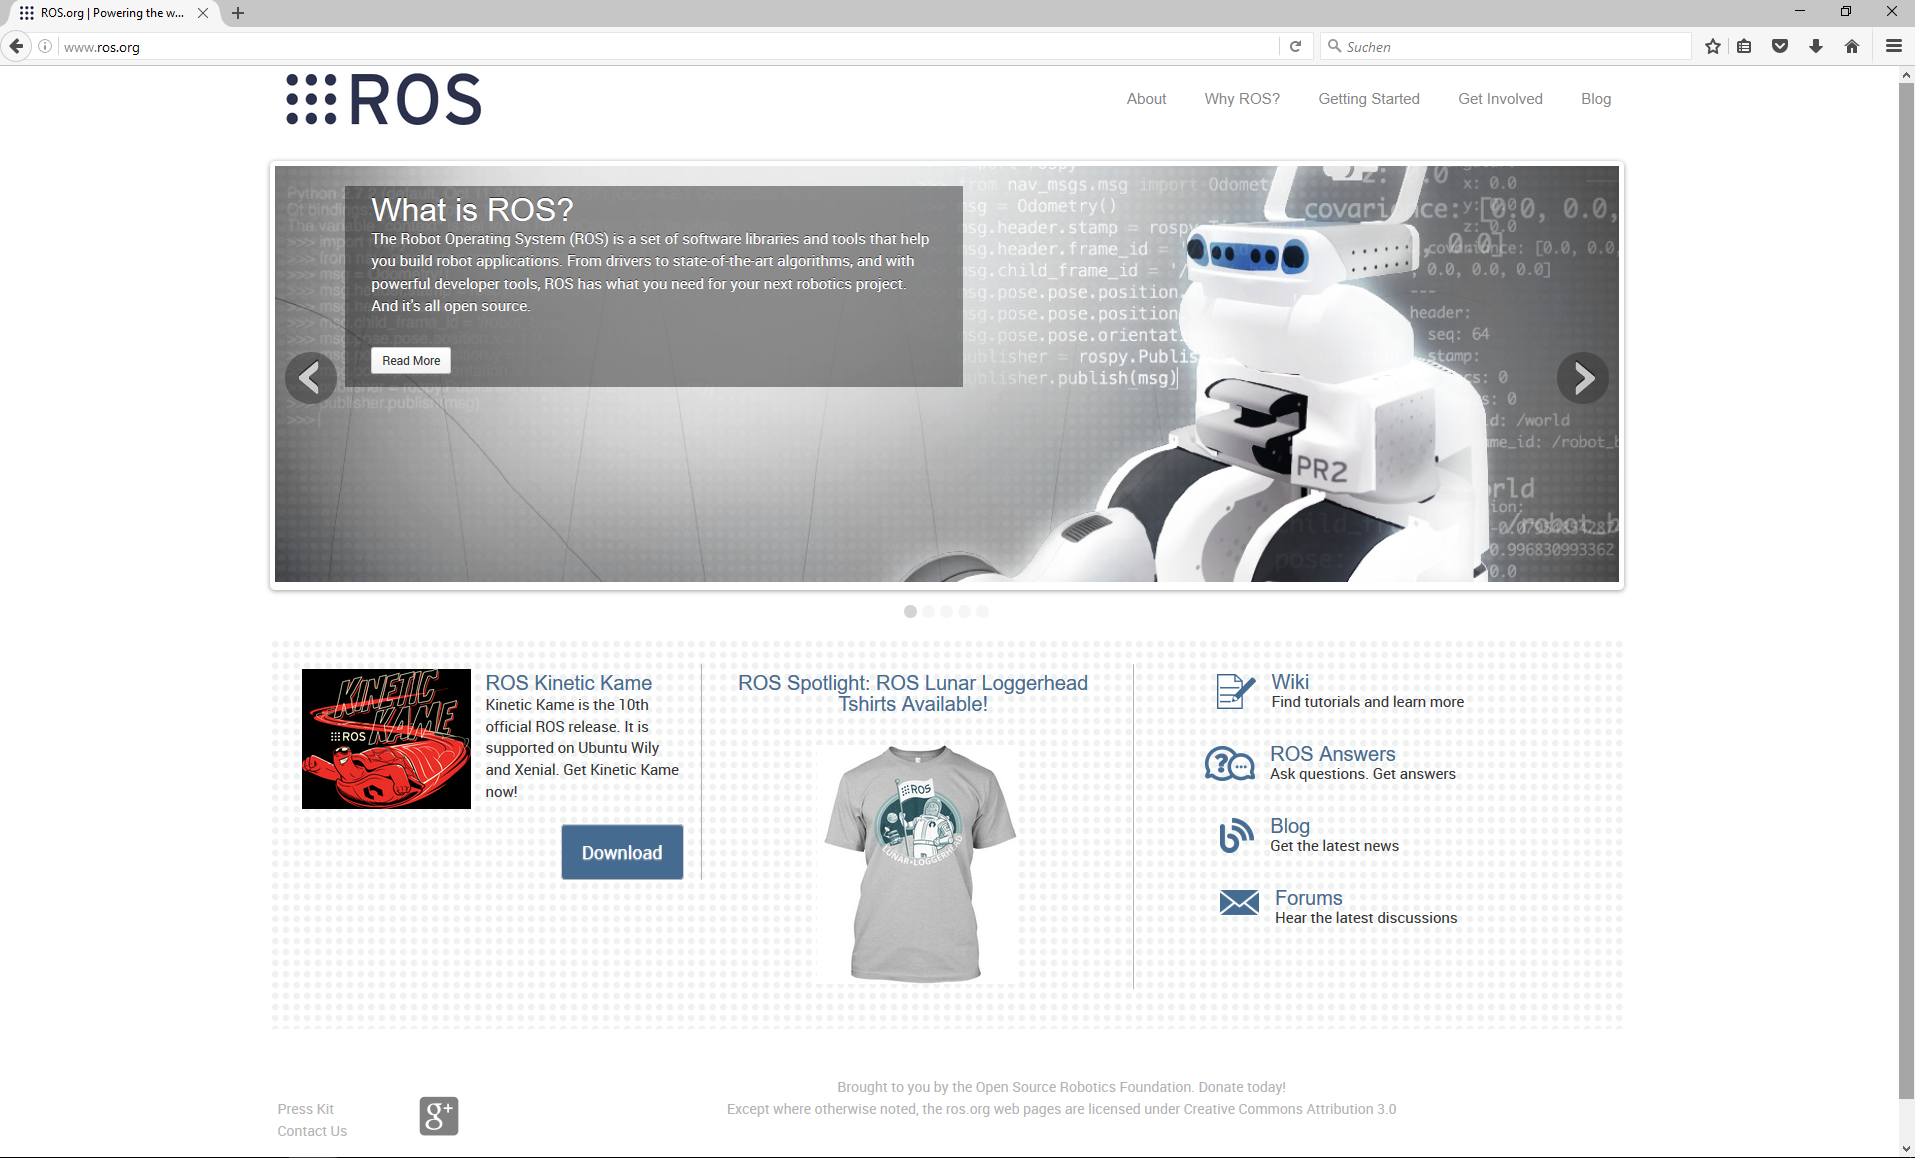
\includegraphics[width=1.5\textwidth]{./Abbildungen/ros_screenshot.png}
    % ros_screenshot.png: 0x0 pixel, 300dpi, 0.00x0.00 cm, bb=
    
    \end{column}
   \end{columns}
  \end{frame}

  \begin{frame}
   \frametitle{Graph-based communication layer}
   \begin{columns}[onlytextwidth]
    \begin{column}{0.5\textwidth}
    
      \begin{description}
       \item [\textbf{Node}] software module, process
       \item [\textbf{Messages}] data in a predefined structure
       \item [\textbf{Topic}] where messages go through
       \item [\textbf{Service}] allows synchronous communication (request / response)
      \end{description}
       
    \end{column}
    \begin{column}{0.5\textwidth}

    \begin{figure}[h]
      \centering
      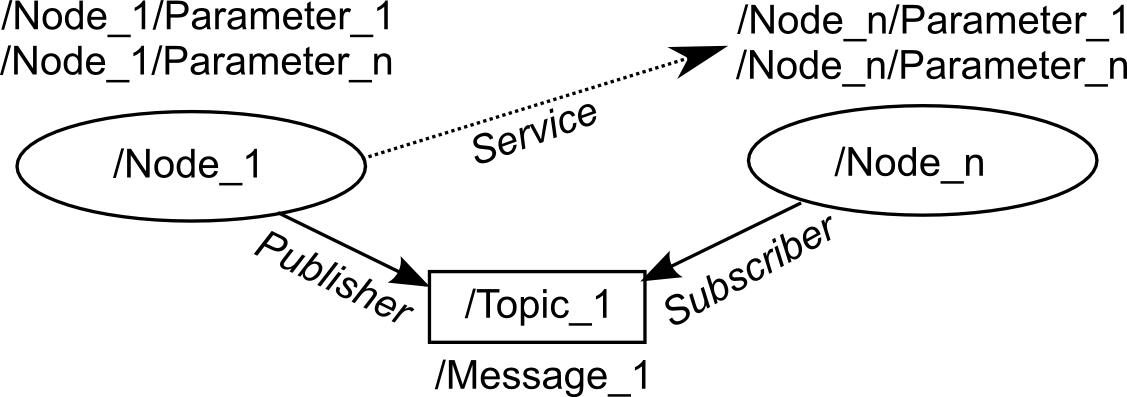
\includegraphics[width=\textwidth]{./Abbildungen/ROS-Graph-basic.png}
      % ROS-Graph-basic.png: 0x0 pixel, 300dpi, 0.00x0.00 cm, bb=
      \caption{ROS communication principle}
      \label{abb:graph}
    \end{figure}
% TODO insert Figure with communication layer
    \end{column}
   \end{columns}
  \end{frame}

\section{Implemented Acquistion Software}

\section{Conclusion and Outlook}




% %----------------------------------------------------------------------------------------
% % Listings mit Python-Code
% \defverbatim[colored]\lstOne{
% \begin{lstlisting}[language=python,basicstyle=\ttfamily,keywordstyle=\color{blue}]
% #!/usr/bin/env python
% import rospy
% from std_msgs.msg import String
% 
% def talker():
%     [...]
% 
% if __name__ == '__main__':
%     try:
%         talker()
%     except rospy.ROSInterruptException:
%         pass
% \end{lstlisting}
% }
% 
% \defverbatim[colored]\lstTwo{
% \begin{lstlisting}[language=python,basicstyle=\ttfamily,keywordstyle=\color{blue}]
% [...]
% def talker():
%     pub = rospy.Publisher('chatter', \ 
%     String, queue_size=10)
%     rospy.init_node('talker')
%     rate = rospy.Rate(10) # 10hz
%     while not rospy.is_shutdown():
%         hello_str = "hello world %s" \
%         % rospy.get_time()
%         pub.publish(hello_str)
%         rate.sleep()
% [...]
% \end{lstlisting}
% }
% 
% \defverbatim[colored]\lstThree{
% \begin{lstlisting}[language=python,basicstyle=\ttfamily,keywordstyle=\color{blue}]
% #!/usr/bin/env python
% import rospy
% from std_msgs.msg import String
% 
% def callback(data):
%     rospy.loginfo(rospy.get_caller_id() + \
%     "I heard %s", data.data)  
% def listener():
%     rospy.init_node('listener')
%     rospy.Subscriber("chatter", String, \
%     callback)
%     rospy.spin()
% if __name__ == '__main__':
%     listener()
% \end{lstlisting}
% }
%--------------------------------------------------------------------------------

% % TITELSEITE
% \begin{frame}
%  \titlepage
% \end{frame}
% 
% % WAS IST ROS
% \section{Was ist ROS?}
% \begin{frame}
% \frametitle{Was ist ROS?}
% \begin{itemize}
%  \item Robotic Operating System (ROS)
%  \item Flexibles Framework für die Robotiksoftwareentwicklung
%  \item FOSS (freie Open Source-Software)
%  \item Ubuntu
%  \item Weite Verbreitung (in der Robotik-Community)
%  \item Modulares Design
%  \item Graph-basiertes Kommunikationskonzept (Synchron und Asynchron)
%  \item Breite Sensorunterstützung
%  \item Mächtige Tools
% \end{itemize}
% \end{frame}
% 
% % graph-basiertes Kommunikationskonzept
% \section{Graph-basiertes Kommunikationskonzept}
% \begin{frame}
%  \frametitle{Graph-basiertes Kommunikationskonzept}
% \begin{figure}[h!]
%  \centering
%  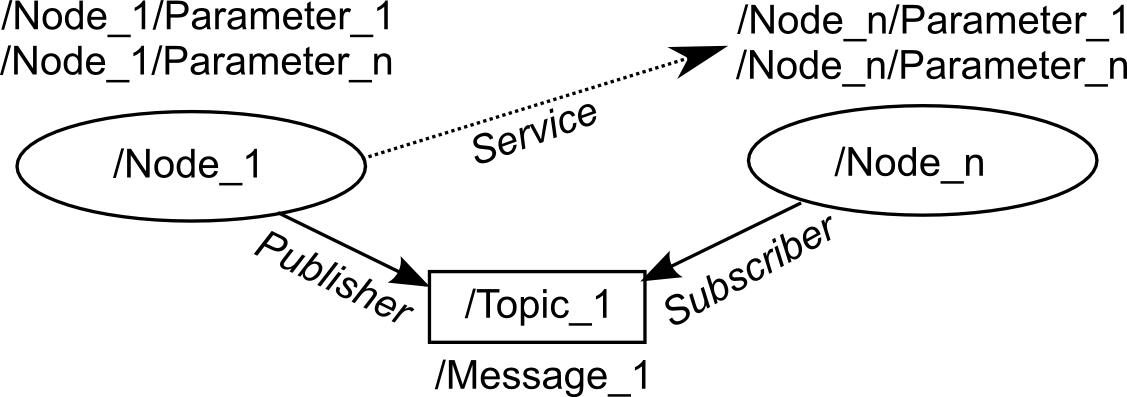
\includegraphics{./Abbildungen/ROS-Graph-basic.png}
%  % ROS-Graph-basic.png: 1127x397 pixel, 300dpi, 9.54x3.36 cm, bb=0 0 270 95
%  \caption{ROS-Kommunikationskonzept}
%  \label{abb:ROSCOM}
% \end{figure}
% 
% 
% \end{frame}
% 
% % Publisher
% \section{Publisher}
% \begin{frame}
%  \frametitle{Node mit «Hello World»-Publisher}
%   \lstOne
% \end{frame}
% 
% \begin{frame}
%  \frametitle{Node mit «Hello World»-Publisher}
%   \lstTwo
% \end{frame}
% 
% % Subscriber
% \section{Subscriber}
% \begin{frame}
%  \frametitle{Node mit «Hello World»-Subscriber}
%  \lstThree
% \end{frame}
% 
% \begin{frame}
%  \frametitle{Video Hello World-Demo}
% \begin{center}
% \movie[showcontrols]{\includegraphics[width=1\textwidth]{./Abbildungen/Video.jpg}}{./Abbildungen/ROSTutorial.mpg}
% \end{center}
%   %\includemovie[autoplay]{4cm}{3cm}{./Abbildungen/ROSTutorial.mpg}
% \end{frame}
% 
% 
% % Anwendungen
% \section{Unterstützung}
% \begin{frame}
%  \frametitle{Hardware-Support}
%  Zahlreiche frei verfügbare Nodes für:
%  \begin{itemize}
%   \item Kameras
%   \item IMUs
%   \item Laserscanner
%   \item Odometer
%   \item Datenvisualisierung
%   \item Steuerung
%   \item ...
%  \end{itemize}
% \begin{figure}[h!]
%  \centering
%  \includegraphics[width=4cm]{./Abbildungen/MMS.jpg}
%  % MMS.jpg: 400x196 pixel, 72dpi, 14.11x6.91 cm, bb=0 0 400 196
%  \caption{Mobile Mapping System des IVGI}
%  \label{abb:MMS}
% \end{figure}
% \end{frame}
% 
% \begin{frame}
% \frametitle{Video SLAM-Demo}
%  \begin{center}
% \movie[showcontrols]{\includegraphics[width=1\textwidth]{./Abbildungen/Video.jpg}}{./Abbildungen/ROSSlam.mp4}
% \end{center}
% \end{frame}
% 
% 
% 
% \section{Fazit}
% % FAZIT
% \begin{frame}
%  \frametitle{Fazit}
%  \begin{itemize}
%   \item Zusammenstellung von Realtime-Processing-Pipelines dank modularem Aufbau
%   \item Hohe Flexibilität
%   \item Weite Verbreitung
%   \item Schnelle Entwicklung mit Python
%   \item Einsatz für Robotik-Anwendungen und Multisensorsystemen
%  \end{itemize}
% 
% \end{frame}
% 
% \begin{frame}
% 
% \textbf{ Danke für Ihre Aufmerksamkeit!}
% \begin{figure}[h!]
%  \centering
%  \includegraphics[height=4cm]{./Abbildungen/stair.jpg}
%  % stair.jpg: 782x1650 pixel, 72dpi, 27.59x58.21 cm, bb=0 0 782 1650
%  \caption{Erster Roboter mit ROS: STanford Artificial Intelligence Robot}
%  \label{abb:Stair}
% \end{figure}
% 
% \end{frame}




\end{document}
